\documentclass[11pt,oneside]{article}

\usepackage[a4paper,margin=26mm,headheight=23pt]{geometry}
\usepackage[T1]{fontenc}
\usepackage[utf8]{inputenc}
\IfFileExists{libertinus.sty}{\usepackage{libertinus}}{\usepackage{lmodern}}
\usepackage[final]{microtype}
\usepackage{amsmath,amssymb,amsthm,mathtools,mathrsfs,bm}
\usepackage{booktabs,longtable,tabularx,array,multirow}
\usepackage{graphicx}
\usepackage{xcolor}
\usepackage{enumitem}
\usepackage{fancyhdr}
\usepackage{titlesec}
\usepackage[most]{tcolorbox}
\usepackage{listings}
\usepackage{fvextra}
\usepackage{xurl}
\usepackage{hyperref}
\usepackage[capitalise,nameinlink,noabbrev]{cleveref}
\usepackage{needspace}

\definecolor{ink}{HTML}{17212B}
\definecolor{navy}{HTML}{173B57}
\definecolor{teal}{HTML}{167D83}
\definecolor{gold}{HTML}{A66F12}
\definecolor{softblue}{HTML}{EDF4F8}
\definecolor{softteal}{HTML}{ECF7F6}
\definecolor{softgold}{HTML}{FBF5E8}
\definecolor{softred}{HTML}{FAEEEE}
\definecolor{rulegray}{HTML}{D6DEE3}
\definecolor{codegray}{HTML}{F4F6F7}

\hypersetup{
  colorlinks=true,
  linkcolor=navy,
  citecolor=teal,
  urlcolor=teal,
  pdftitle={Zero-Divisor-Preserving q-Richardson Extrapolation for the Fabius--Rvachev Sinc Product},
  pdfauthor={Research report prepared for Vladimir Reshetnikov},
  pdfsubject={Fabius function, Rvachev up-function, Thue--Morse sequence, q-binomial Richardson extrapolation, infinite sinc products},
  pdfkeywords={Fabius function, Rvachev up-function, Thue-Morse, q-binomial, Richardson extrapolation, sinc product, Lambert W, Bell polynomials, Bernoulli numbers}
}
\urlstyle{same}

\setlength{\parindent}{1.25em}
\setlength{\parskip}{0.16em}
\setlength{\emergencystretch}{2em}
\setlist{itemsep=0.24em,topsep=0.45em,leftmargin=1.75em}
\setcounter{tocdepth}{2}
\setcounter{secnumdepth}{3}
\allowdisplaybreaks[2]
\numberwithin{equation}{section}

\titleformat{\section}{\Large\bfseries\color{navy}}{\thesection}{0.75em}{}
\titleformat{\subsection}{\large\bfseries\color{teal}}{\thesubsection}{0.65em}{}
\titleformat{\subsubsection}{\normalsize\bfseries\color{ink}}{\thesubsubsection}{0.55em}{}
\titlespacing*{\section}{0pt}{2.4ex plus .5ex minus .2ex}{1.1ex}
\titlespacing*{\subsection}{0pt}{1.8ex plus .4ex minus .2ex}{0.7ex}

\pagestyle{fancy}
\fancyhf{}
\fancyhead[L]{\small\color{navy}Zero-preserving $q$-Richardson extrapolation}
\fancyhead[R]{\small\color{teal}\nouppercase{\leftmark}}
\fancyfoot[C]{\small\thepage}
\renewcommand{\headrulewidth}{0.35pt}
\renewcommand{\headrule}{\hbox to\headwidth{\color{rulegray}\leaders\hrule height \headrulewidth\hfill}}

\newtheoremstyle{frontier}
  {0.8em}{0.8em}{\itshape}{} {\bfseries\color{navy}}{.}{0.55em}{}
\theoremstyle{frontier}
\newtheorem{theorem}{Theorem}[section]
\newtheorem{proposition}[theorem]{Proposition}
\newtheorem{lemma}[theorem]{Lemma}
\newtheorem{corollary}[theorem]{Corollary}
\newtheorem{conjecture}[theorem]{Conjecture}
\newtheorem{problem}[theorem]{Problem}
\theoremstyle{definition}
\newtheorem{definition}[theorem]{Definition}
\newtheorem{algorithm}[theorem]{Algorithm}
\newtheorem{example}[theorem]{Example}
\theoremstyle{remark}
\newtheorem{remark}[theorem]{Remark}
\newtheorem{warning}[theorem]{Warning}

\crefname{theorem}{theorem}{theorems}
\crefname{proposition}{proposition}{propositions}
\crefname{lemma}{lemma}{lemmas}
\crefname{corollary}{corollary}{corollaries}
\crefname{conjecture}{conjecture}{conjectures}
\crefname{problem}{problem}{problems}
\crefname{definition}{definition}{definitions}
\crefname{algorithm}{algorithm}{algorithms}
\crefname{example}{example}{examples}
\crefname{remark}{remark}{remarks}

\newtcolorbox{statusbox}[1][]{
  enhanced,breakable,colback=softblue,colframe=navy,
  boxrule=0.6pt,arc=2pt,left=7pt,right=7pt,top=6pt,bottom=6pt,
  title={#1},fonttitle=\bfseries
}
\newtcolorbox{resultbox}[1][]{
  enhanced,breakable,colback=softteal,colframe=teal,
  boxrule=0.6pt,arc=2pt,left=7pt,right=7pt,top=6pt,bottom=6pt,
  title={#1},fonttitle=\bfseries
}
\newtcolorbox{cautionbox}[1][]{
  enhanced,breakable,colback=softgold,colframe=gold,
  boxrule=0.6pt,arc=2pt,left=7pt,right=7pt,top=6pt,bottom=6pt,
  title={#1},fonttitle=\bfseries
}
\newtcolorbox{frontierbox}[1][]{
  enhanced,breakable,colback=softred,colframe=red!65!black,
  boxrule=0.6pt,arc=2pt,left=7pt,right=7pt,top=6pt,bottom=6pt,
  title={#1},fonttitle=\bfseries
}

\lstdefinestyle{frontiercode}{
  language=Python,
  basicstyle=\ttfamily\footnotesize,
  backgroundcolor=\color{codegray},
  frame=single,
  rulecolor=\color{rulegray},
  breaklines=true,
  columns=fullflexible,
  showstringspaces=false,
  keywordstyle=\color{navy}\bfseries,
  commentstyle=\color{teal},
  stringstyle=\color{gold!80!black},
  xleftmargin=0.6em,xrightmargin=0.6em,
  aboveskip=0.8em,belowskip=0.8em
}

\newcommand{\sinc}{\operatorname{sinc}}
\newcommand{\Log}{\operatorname{Log}}
\newcommand{\Up}{\operatorname{up}}
\newcommand{\ord}{\operatorname{ord}}
\newcommand{\sgn}{\operatorname{sgn}}
\newcommand{\Res}{\operatorname*{Res}}
\newcommand{\Li}{\operatorname{Li}}
\newcommand{\Var}{\operatorname{Var}}
\newcommand{\E}{\mathbb E}
\newcommand{\N}{\mathbb N}
\newcommand{\Z}{\mathbb Z}
\newcommand{\R}{\mathbb R}
\newcommand{\C}{\mathbb C}
\newcommand{\dd}{\,\mathrm d}
\newcommand{\e}{\mathrm e}
\newcommand{\ii}{\mathrm i}
\newcommand{\eps}{\varepsilon}
\newcommand{\bigO}{\mathrm O}
\newcommand{\smallo}{\mathrm o}
\newcommand{\vtwo}{\nu_2}
\newcommand{\wt}{s_2}
\newcommand{\qpoch}[2]{(#1;#2)}
\newcommand{\qbinom}[2]{\genfrac{[}{]}{0pt}{}{#1}{#2}_{q}}
\newcommand{\abs}[1]{\left|#1\right|}
\newcommand{\norm}[1]{\left\lVert#1\right\rVert}
\newcommand{\doi}[1]{\href{https://doi.org/#1}{doi:#1}}
\newcommand{\repo}{\url{https://github.com/VladimirReshetnikov/ProveIt/tree/main/Analysis/FabiusFunction/docs}}
\newcommand{\commitsha}{\nolinkurl{7f4e6e6fdd57f756f303b20f56b5382627e5e1d4}}

\begin{document}
\hypersetup{pageanchor=false}

\begin{titlepage}
\centering
\vspace*{1.2cm}
{\color{navy}\rule{0.84\textwidth}{1.2pt}}\\[1.0cm]
{\Huge\bfseries\color{navy} Zero-Divisor-Preserving\\[0.16em]
$q$-Richardson Extrapolation\par}
\vspace{0.35cm}
{\LARGE\bfseries\color{ink} for the Fabius--Rvachev Sinc Product\par}
\vspace{0.75cm}
{\Large\color{teal}Exact same-parity nesting thresholds, holomorphic continuation through zeros,\\
and certified local spectral jets\par}
\vspace{1.0cm}
{\color{navy}\rule{0.84\textwidth}{0.6pt}}\\[1.2cm]

\begin{minipage}{0.86\textwidth}
\large
A frontier report based on a recursive audit of all 68 \texttt{*.tex} sources under
\path{Analysis/FabiusFunction/docs}, including current expositions, active frontier drafts,
archived revisions, Fourier-decay audits, and transcribed source papers.  The report starts
where the latest repository drafts stop: it resolves their open same-parity nesting problem
and removes the logarithmic extrapolator's apparent obstruction at zeros by factoring the
finite zero divisor before extrapolating the zero-free tail.
\end{minipage}

\vfill
{\large Research synthesis prepared for Vladimir Reshetnikov\par}
\vspace{0.25cm}
{\large 27 August 2026\par}
\vspace{0.65cm}
{\small Repository snapshot: \commitsha\par}
\end{titlepage}

\hypersetup{pageanchor=true}
\pagenumbering{roman}

\begin{abstract}
Let
\[
 P_b(t)=\prod_{k\ge1}\sinc\!\left(\frac{t}{b^k}\right),
 \qquad \sinc z=\frac{\sin z}{z},\qquad b>1,
\]
and put $q=b^{-2}$.  The inspected repository already develops exact logarithmic
$q$-Richardson extrapolation for finite sections of this product.  Its transform has
alternating error sign and a complete Bernoulli--zeta/Bell-polynomial expansion, but the
logarithmic definition is stated only away from the zeros; the same source leaves
monotonicity between extrapolants of the same parity as an open parameter-classification
problem.

Both gaps are closed here.  For the prefix $P_{b,N}$, the omitted tail is zero-free in the
natural disk $|t|<\pi b^{N+1}$.  We extrapolate analytic logarithms of the \emph{relative
partial tails} and then multiply by $P_{b,N}$.  The resulting factorized transform is
holomorphic across every prefix zero, preserves the complete zero divisor with
multiplicity, and agrees with the earlier multiplicative transform wherever the latter is
defined.  Its quotient by $P_b$, after cancellation of common zeros, is exactly
$\exp(E_{N,r})$, where
\[
 E_{N,r}(t)=(-1)^r\frac{q^{r(r+1)/2}}{(q;q)_r}
 \sum_{m\ge r+1}\frac{\zeta(2m)}{m}
 \frac{(q^{m-r};q)_r}{1-q^m}
 \left(\frac{t}{\pi b^{N+1}}\right)^{2m}.
\]
Consequently, the alternating brackets survive at zeros as certified brackets for the first
nonzero derivative, and Cauchy estimates certify every coefficient of the zero-normalized
local germ.

Write $M_r(q,a)=|E_{N,r}|$ after replacing the final even power by $a^m$, $0<a<1$.
The exact classification proved here is
\[
 M_{r+2}(q,a)<M_r(q,a)\quad\hbox{for every }0<a<1
 \quad\Longleftrightarrow\quad q^{r+1}(1+q)\le1.
\]
If the inequality fails, the two same-parity errors cross exactly once.  The proof is
coefficientwise: the shared-coefficient ratio is strictly increasing in $m$ and tends to
$q^{2r+3}/((1-q^{r+1})(1-q^{r+2}))$.  Thus all levels are nested from order zero exactly
when $q\le(\sqrt5-1)/2$, or equivalently $b\ge\sqrt\varphi$.  In the dyadic Fabius--Rvachev
case $q=1/4$, every level is nested.  This gives two monotone analytic chains squeezing the
Fourier product while preserving all included integer zeros, their multiplicities
$1+\nu_2(n)$, their Thue--Morse lobe signs, and their first nonzero derivatives.

Numerical experiments, supplied as a fully commented Python program, independently compare
direct products with the exact coefficient series, compute the threshold curve and unique
crossings, and demonstrate derivative-ratio errors below $10^{-24}$ at the multiplicity-five
zero $x=48$ by order eight.  The final sections formulate conjectures and a formalization
program for general refinement masks, complex boundary continuation, optimal finite
precision, inverse-Fabius coupling, and periodically perturbed Lambert saddles.
\end{abstract}

\begin{statusbox}[Proof and novelty status]
\textbf{Established inputs from the repository.}  The Fabius/Rvachev identities; exact
dyadic arithmetic; Thue--Morse, $q$-binomial, Bernoulli, Bell, Lambert-$W$, and inverse
asymptotic machinery; the infinite sinc product and its integer zero multiplicities; the
$q$-Lagrange weights; the exact transformed logarithmic tail series; alternating error
sign; bounded weight condition number; phase-locked endpoint Richardson transforms; and the
large Fourier-decay theory are treated in the inspected corpus.

\textbf{Proved in this report.}  The factorized zero-divisor-preserving transform; its
holomorphic extension through all included zeros; exact zero-normalized quotient and local
jet identities; complex nonasymptotic bounds; the necessary-and-sufficient same-parity
nesting criterion; uniqueness and analyticity of the supercritical crossing; the
$\sqrt\varphi$ base threshold; large-order threshold asymptotics; and the nested dyadic
spectral-jet brackets.

\textbf{Not claimed.}  ``New'' means not found in the recursively inspected repository or
in the targeted primary-source searches described in \cref{sec:literature}.  It is not an
unqualified assertion of worldwide priority.  None of the new theorems is claimed to have
a Lean counterpart at the snapshot commit.
\end{statusbox}

\clearpage
\tableofcontents
\clearpage
\pagenumbering{arabic}

\section{Corpus boundary, audit method, and collision control}\label{sec:audit}

\subsection{Pinned recursive corpus}

The analysis is pinned to commit \commitsha.  This matters because the active frontier
subtree was changing during the work: the GitHub code-search index lagged the tree, while the
recursive Git objects gave the exact count of 68 TeX files.  Their complete path manifest is
reproduced in \cref{app:manifest} and supplied as a machine-readable text file in the
archive.

\begin{center}
\begin{tabularx}{\textwidth}{@{}l r X@{}}
\toprule
Stratum & Files & Audit role\\
\midrule
Living expositions and synthesis & 5 & Formalization-backed baseline, glossary,
non-elementarity, Lean map, and consolidated frontier volume.\\
Active frontier drafts & 24 & Arithmetic rays, half-integer spectra, inverse asymptotics,
Pascal--Rvachev hierarchies, zero determinants, $q$-Richardson analysis, and twelve
Fourier-decay reports/audits.\\
Frozen archive & 32 & Revision history, early notes, superseded expositions, prior
$q$-calculus articles, convergence studies, and source provenance.\\
Transcribed source papers & 7 & Arias de Reyna, Aistleitner--Hofer--Larcher, Toth,
Allouche--Shallit, and related primary context.\\
\midrule
Total & 68 & Every recursive \texttt{*.tex} path at the pinned commit.\\
\bottomrule
\end{tabularx}
\end{center}

Archived files were not treated as 32 independent current papers.  They were read as a
revision graph: distinctive claims were checked against the current descendant and the
archive's own consolidation/provenance maps.  The twelve Fourier documents were similarly
read as two waves plus two comparative audits, so a superseded constant or conjecture could
not be mistaken for the current state of the problem.

\subsection{The mature baseline}

The corpus is unusually dense.  Among other things, it already contains:
\begin{enumerate}
\item a proof-oriented primary exposition of the bounded Fabius function, Rvachev's compact
      up-function, and the signed global extension, with exact separation of those objects;
\item probability, convolution, spline, Fourier, moment, exact dyadic, $q$-binomial, and
      Thue--Morse representations;
\item a quadratic-plus-periodic negative-Laplace exponent, lower-branch Lambert phase,
      all-orders endpoint and inverse expansions, closed inverse jets, and Bell-polynomial
      coefficient transfer;
\item finite geometric-grid Richardson filters with exact Gaussian $q$-binomial weights,
      alternating logarithmic brackets, complete transformed tail coefficients, and bounded
      condition number;
\item integer-zero spectral determinants, exact multiplicities, half-integer spectral
      arithmetic, Prouhet quadrature, rational dyadic rays, cyclotomic orbit norms, and a
      Pascal--Rvachev hierarchy;
\item a two-wave analysis of pointwise, metric, extremal, quadratic-mean, Ces\`aro, and
      shell-adaptive Fourier decay.
\end{enumerate}
The main challenge was therefore not producing another list of identities.  It was finding a
statement that survives comparison with the newest same-day drafts.

\subsection{Candidates deliberately discarded}

Several promising-looking ideas were rejected after exact comparison:
\begin{itemize}
\item phase-locked reciprocal-grid Richardson extrapolation for the Lambert saddle was
      already present, including its complete homogeneous and Bell-polynomial moments;
\item the integer zero divisor, spectral zeta, heat trace, local all-order zero jets, and
      $q$-deformation already had a dedicated report;
\item arithmetic rational rays and half-integer weighted Prouhet formulae had newer active
      treatments;
\item generic log-periodic Fourier envelopes and transfer-operator constants were covered by
      the comparative audits;
\item the $q$-Pochhammer/Thue--Morse dictionary for endpoint corrections and Fourier-zero
      multiplicities was already developed in the spectral-endpoint report.
\end{itemize}

\begin{resultbox}[The two surviving openings]
The latest $q$-Richardson draft explicitly leaves two questions open: whether same-parity
brackets are monotone in identifiable parameter regimes, and how the logarithmic transform
should be continued across zeros.  The present report resolves both questions exactly.
\end{resultbox}

\subsection{External literature boundary}\label{sec:literature}

The external search was used to prevent reinvention of standard extrapolation theory and to
locate adjacent product-approximation work.  Generalized Richardson theory on geometric
meshes, including convergence and stability, is classical \cite{sidi1996,sidi-siam}.  The
$q$-binomial identities used to write the weights belong to standard basic hypergeometric
calculus \cite{gasper-rahman}.  The Lambert function and its branch asymptotics are standard
\cite{corless}.  The Fabius/Rvachev baseline comes from Arias de Reyna and related work
\cite{arias-function,arias-arithmetic,haugland}, while the lacunary product's metric theory
is represented by Aistleitner--Hofer--Larcher \cite{ahl2017}.

Targeted searches located recent Pad\'e work for products of functions, but not a construction
that factors a finite canonical zero divisor and applies geometric $q$-Richardson
extrapolation to the zero-free infinite tail, nor the exact threshold in
\cref{thm:nesting-classification}.  The nearest classical results concern extrapolation of
asymptotic scales, not preservation of an entire function's moving zero divisor.

\section{Established logarithmic \texorpdfstring{$q$}{q}-Richardson structure}\label{sec:baseline}

\subsection{The lacunary sinc product}

Fix $b>1$ and set
\begin{equation}
 q=b^{-2}\in(0,1).
 \label{eq:qdef}
\end{equation}
We use the entire normalized sinc function
\[
 \sinc z=\begin{cases}\sin z/z,&z\ne0,\\1,&z=0,
 \end{cases}
\]
and define
\begin{equation}
 P_b(t)=\prod_{k=1}^{\infty}\sinc\!\left(\frac{t}{b^k}\right),
 \qquad
 P_{b,N}(t)=\prod_{k=1}^{N}\sinc\!\left(\frac{t}{b^k}\right).
 \label{eq:Pb}
\end{equation}
Uniform convergence on compact sets makes $P_b$ entire.  The first omitted factor has its
nearest zeros at $\pm\pi b^{N+1}$, so the natural tail disk is
\begin{equation}
 D_N=\{t\in\C:|t|<\pi b^{N+1}\}.
 \label{eq:DN}
\end{equation}
Define the complete and partial relative tails directly by their products:
\begin{equation}
 T_N(t)=\prod_{k=N+1}^{\infty}\sinc\!\left(\frac{t}{b^k}\right)
       =P_b\!\left(\frac{t}{b^N}\right),
 \qquad
 T_{N,j}(t)=\prod_{k=N+1}^{N+j}\sinc\!\left(\frac{t}{b^k}\right),\quad j\ge0,
 \label{eq:tails}
\end{equation}
with the empty product $T_{N,0}=1$.  These total functions satisfy
$P_b=P_{b,N}T_N$ and $P_{b,N+j}=P_{b,N}T_{N,j}$ everywhere.  Only where
$P_{b,N}(t)\ne0$ do we also write them as the quotients
$T_N=P_b/P_{b,N}$ and $T_{N,j}=P_{b,N+j}/P_{b,N}$.

\begin{lemma}[Zero-free tail disk]\label{lem:zero-free-tail}
Every $T_{N,j}$, including $T_N$, is holomorphic and zero-free on $D_N$.  It therefore has a
unique holomorphic logarithm on $D_N$ normalized to vanish at $t=0$.  On
$D_N\cap\R$, all these tails are positive.
\end{lemma}

\begin{proof}
Every zero of $\sinc(t/b^k)$ has modulus at least $\pi b^k$.  For $k\ge N+1$
this is at least the radius of $D_N$, with equality only for the first omitted factor and only
on the boundary.  Thus every finite relative tail and the locally uniform infinite tail are
zero-free in the disk.  The disk is simply connected, giving the normalized logarithm.
For real $|t|<\pi b^{N+1}$ every omitted argument has modulus less than $\pi$, where
$\sin x/x>0$.
\end{proof}

\subsection{Bernoulli--zeta coefficients}

For $|z|<\pi$,
\begin{equation}
 -\log\sinc z
 =\sum_{m=1}^{\infty}\frac{\zeta(2m)}{m\pi^{2m}}z^{2m}
 =\sum_{m=1}^{\infty}
   \frac{(-1)^{m+1}2^{2m-1}B_{2m}}{m(2m)!}z^{2m}.
 \label{eq:log-sinc}
\end{equation}
Consequently, with
\begin{equation}
 u_N(t)=\frac{t}{\pi b^{N+1}},
 \label{eq:uN}
\end{equation}
one has the exact prefix error
\begin{equation}
 \Log P_{b,N}(t)-\Log P_b(t)
 =\sum_{m\ge1}\frac{\zeta(2m)}{m(1-q^m)}u_N(t)^{2m}
 \label{eq:prefix-log-error}
\end{equation}
whenever both logarithms are taken on a zero-free component.  The right side itself is
holomorphic throughout $D_N$ and will be the invariant object used below.

\subsection{Geometric Lagrange weights}

For $r\ge0$, let $\lambda_{r,j}(q)$ be the Lagrange interpolation weights at nodes
$1,q,\ldots,q^r$, evaluated at the origin:
\begin{equation}
 \lambda_{r,j}(q)
 =\frac{(-1)^{r-j}q^{(r-j)(r-j+1)/2}}
       {(q;q)_j(q;q)_{r-j}},
 \qquad 0\le j\le r,
 \label{eq:weights}
\end{equation}
where $(a;q)_n=\prod_{k=0}^{n-1}(1-aq^k)$.  Their transformed moments are
\begin{equation}
 S_{r,m}(q)=\sum_{j=0}^{r}\lambda_{r,j}(q)q^{jm}
 =\begin{cases}
 1,&m=0,\\
 0,&1\le m\le r,\\
 \displaystyle
 (-1)^r\frac{q^{r(r+1)/2}(q^{m-r};q)_r}{(q;q)_r},&m\ge r+1.
 \end{cases}
 \label{eq:transformed-moments}
\end{equation}
This is the finite $q$-binomial cancellation mechanism already developed in the repository.

Away from zeros, the existing multiplicative transform can be written schematically as
\[
 \exp\!\left(\sum_{j=0}^{r}\lambda_{r,j}\Log P_{b,N+j}\right).
\]
Its exact logarithmic error and alternating sign are established there.  The obstruction is
that no single logarithm of $P_{b,N+j}$ can pass through a zero.  The next section removes
that obstruction without changing the transform where it was already defined.

\section{Factorization through the complete zero divisor}\label{sec:factorized}

\subsection{Definition and holomorphic continuation}

\begin{definition}[Factorized tail transform]\label{def:factorized}
On $D_N$, let $\Log T_{N,j}$ be the normalized logarithms from
\cref{lem:zero-free-tail}.  Define
\begin{align}
 \widehat T_{N,r}(t)
   &=\exp\!\left(\sum_{j=0}^{r}\lambda_{r,j}(q)\Log T_{N,j}(t)\right),
 \label{eq:hat-tail}\\
 \widehat P^{\mathrm{fac}}_{b,N,r}(t)
   &=P_{b,N}(t)\widehat T_{N,r}(t).
 \label{eq:hat-factorized}
\end{align}
\end{definition}

The superscript ``fac'' will usually be suppressed once no confusion with the unfactored
logarithmic expression is possible.

\begin{theorem}[Zero-divisor-preserving continuation]\label{thm:zero-preserving}
For every $N,r\ge0$:
\begin{enumerate}
\item $\widehat P^{\mathrm{fac}}_{b,N,r}$ is holomorphic on $D_N$.
\item Wherever $P_{b,N}$ is nonzero, it agrees with the earlier multiplicative
      $q$-Richardson transform formed from $P_{b,N},\ldots,P_{b,N+r}$.
\item $P_b$, $P_{b,N}$, and $\widehat P^{\mathrm{fac}}_{b,N,r}$ have exactly the same zero
      divisor in $D_N$, including multiplicities.
\item After cancellation of that common zero divisor, the quotient
      $\widehat P^{\mathrm{fac}}_{b,N,r}/P_b$ extends to a holomorphic zero-free function on
      all of $D_N$.
\end{enumerate}
\end{theorem}

\begin{proof}
The function $\widehat T_{N,r}$ is an exponential of a holomorphic function and is therefore
holomorphic and zero-free.  This proves the first assertion after multiplication by the
finite prefix.

If $P_{b,N}(t)\ne0$, then
\[
 \Log P_{b,N+j}=\Log P_{b,N}+\Log T_{N,j}
\]
on the locally normalized branch.  Since $\sum_j\lambda_{r,j}=1$, the unfactored weighted
logarithm equals $\Log P_{b,N}+\sum_j\lambda_{r,j}\Log T_{N,j}$, proving agreement.

By \cref{lem:zero-free-tail}, both the exact tail $T_N$ and the extrapolated tail
$\widehat T_{N,r}$ are zero-free in $D_N$.  Thus every zero of either full product comes
from $P_{b,N}$ with unchanged multiplicity.  Finally,
\[
 \frac{\widehat P^{\mathrm{fac}}_{b,N,r}}{P_b}
 =\frac{\widehat T_{N,r}}{T_N}
\]
after cancellation, and the right side is holomorphic and zero-free.
\end{proof}

\begin{remark}
The construction is not a numerical patch at a real zero.  It is a holomorphic factorization
on the full complex disk $D_N$.  The finite prefix is a canonical carrier of the entire zero
divisor visible at scale $N$; only the zero-free determinant tail is extrapolated.
\end{remark}

\subsection{Exact error on the whole disk}

\begin{theorem}[Exact zero-normalized logarithmic error]\label{thm:exact-error}
On $D_N$,
\begin{equation}
 \frac{\widehat P^{\mathrm{fac}}_{b,N,r}(t)}{P_b(t)}
 =\exp(E_{N,r}(t))
 \label{eq:quotient-error}
\end{equation}
after cancellation at common zeros, where
\begin{equation}
 \boxed{
 E_{N,r}(t)=(-1)^r\frac{q^{r(r+1)/2}}{(q;q)_r}
 \sum_{m=r+1}^{\infty}\frac{\zeta(2m)}{m}
 \frac{(q^{m-r};q)_r}{1-q^m}
 u_N(t)^{2m}.}
 \label{eq:exact-E}
\end{equation}
In particular,
\begin{equation}
 E_{N,r}(t)
 =(-1)^r\frac{q^{r(r+1)/2}\zeta(2r+2)}
 {(r+1)(1-q^{r+1})}u_N(t)^{2r+2}
 +\bigO(u_N(t)^{2r+4}).
 \label{eq:leading-E}
\end{equation}
\end{theorem}

\begin{proof}
From \eqref{eq:prefix-log-error}, the logarithm of the $j$th relative partial tail is
\[
 \Log T_{N,j}
 =\Log T_N+
 \sum_{m\ge1}\frac{\zeta(2m)}{m(1-q^m)}u_N(t)^{2m}q^{jm}.
\]
Weighting and using $\sum_j\lambda_{r,j}=1$ gives
\[
 \Log\frac{\widehat T_{N,r}}{T_N}
 =\sum_{m\ge1}\frac{\zeta(2m)}{m(1-q^m)}u_N(t)^{2m}S_{r,m}(q).
\]
Insert \eqref{eq:transformed-moments}.  The first $r$ powers vanish, and the remaining
closed form is \eqref{eq:exact-E}.  At $m=r+1$ one has
$(q;q)_r=(q^{m-r};q)_r$, giving \eqref{eq:leading-E}.
\end{proof}

\subsection{Uniform complex bounds}

\begin{proposition}[A computable disk bound]\label{prop:disk-bound}
Let $0<R<\pi b^{N+1}$ and put
\[
 a_R=\left(\frac{R}{\pi b^{N+1}}\right)^2.
\]
Then on $|t|\le R$,
\begin{equation}
 |E_{N,r}(t)|\le B_{N,r}(R)
 :=\frac{q^{r(r+1)/2}}{(q;q)_r}
   \frac{\zeta(2)}{(1-q)(r+1)}
   \frac{a_R^{r+1}}{1-a_R}.
 \label{eq:Bbound}
\end{equation}
Consequently,
\begin{equation}
 \left|\frac{\widehat P^{\mathrm{fac}}_{b,N,r}}{P_b}-1\right|
 \le \e^{B_{N,r}(R)}-1
 \label{eq:relative-bound}
\end{equation}
after zero cancellation, uniformly on the closed disk.
\end{proposition}

\begin{proof}
In \eqref{eq:exact-E}, use
$(q^{m-r};q)_r\le1$, $(1-q^m)^{-1}\le(1-q)^{-1}$,
$\zeta(2m)\le\zeta(2)$, and
\[
 \sum_{m\ge r+1}\frac{a_R^m}{m}
 \le\frac{a_R^{r+1}}{(r+1)(1-a_R)}.
\]
Then use $|\e^z-1|\le\e^{|z|}-1$.
\end{proof}

\subsection{Local jets at every included zero}

\begin{theorem}[Exact spectral-jet quotient]\label{thm:jet-quotient}
Let $t_0\in D_N$ be a zero of $P_b$ of multiplicity $\mu$.  Then
\begin{equation}
 \frac{(\widehat P^{\mathrm{fac}}_{b,N,r})^{(\mu)}(t_0)}
      {P_b^{(\mu)}(t_0)}
 =\exp(E_{N,r}(t_0)).
 \label{eq:first-derivative-ratio}
\end{equation}
More strongly, after removing the common factor $(t-t_0)^\mu$, the quotient of the two
zero-normalized germs is exactly $\exp(E_{N,r}(t))$.  Hence for every $k\ge1$,
\begin{equation}
 \left(\frac{\dd}{\dd t}\right)^k
 \Log\!\left(
 \frac{\widehat P^{\mathrm{fac}}_{b,N,r}(t)/(t-t_0)^\mu}
      {P_b(t)/(t-t_0)^\mu}
 \right)
 =E_{N,r}^{(k)}(t)
 \label{eq:jet-log-derivatives}
\end{equation}
in a neighborhood of $t_0$.
\end{theorem}

\begin{proof}
Write $P_{b,N}(t)=(t-t_0)^\mu A(t)$ with $A(t_0)\ne0$.  Then
\[
 P_b(t)=(t-t_0)^\mu A(t)T_N(t),\qquad
 \widehat P^{\mathrm{fac}}_{b,N,r}(t)=(t-t_0)^\mu A(t)\widehat T_{N,r}(t).
\]
Taking the first nonzero derivative gives the tail ratio; \cref{thm:exact-error} identifies
that ratio with $\exp(E_{N,r}(t_0))$.  Cancelling the complete common germ gives the stronger
identity, and logarithmic differentiation gives \eqref{eq:jet-log-derivatives}.
\end{proof}

\begin{corollary}[Cauchy-certified higher coefficients]\label{cor:cauchy-jets}
Choose $\delta>0$ so that the closed disk $|t-t_0|\le\delta$ lies in $D_N$.  Every Taylor
coefficient of the zero-normalized quotient is bounded explicitly by applying Cauchy's
estimate to $\exp(E_{N,r})-1$ and \cref{prop:disk-bound} on that disk.  More precisely,
$\exp(E_{N,r})\to1$ locally uniformly either as $N\to\infty$ with $r$ fixed, on each fixed
compact set, or as $r\to\infty$ with $N$ fixed, on each compact subset of $D_N$.
Consequently, for every fixed derivative order $k\ge0$, Cauchy's integral formula gives
local uniform convergence of the $k$th derivatives to the $k$th derivative of $1$ (that is,
to $1$ for $k=0$ and to $0$ for $k\ge1$).  No uniformity in the derivative order is claimed.
\end{corollary}

\subsection{Bernoulli and Bell transfer at zeros}

The exponent \eqref{eq:exact-E} is a Bernoulli--zeta series.  Write locally
\[
 E_{N,r}(t)=\sum_{m\ge r+1}e_{r,m}u_N(t)^{2m}.
\]
Then
\begin{equation}
 \exp(E_{N,r}(t))
 =1+\sum_{n\ge r+1}\frac{1}{n!}
 B_n(1!x_1,2!x_2,\ldots,n!x_n)u_N(t)^{2n},
 \label{eq:bell-transfer}
\end{equation}
where $x_m=e_{r,m}$ for $m\ge r+1$ and $x_m=0$ below that order, and $B_n$ is the complete
exponential Bell polynomial.  Bell transfer itself is established in the repository; the new
point is that \eqref{eq:bell-transfer} now applies directly to the ratio of the first nonzero
derivatives and to every zero-normalized local germ.  No separate limiting argument at a zero
is required.

\section{Exact classification of same-parity nesting}\label{sec:nesting}

\subsection{Positive error magnitudes}

For $0<a<1$, define
\begin{equation}
 M_r(q,a)=\frac{q^{r(r+1)/2}}{(q;q)_r}
 \sum_{m=r+1}^{\infty}\frac{\zeta(2m)}{m}
 \frac{(q^{m-r};q)_r}{1-q^m}a^m.
 \label{eq:Mr}
\end{equation}
Thus on the real tail disk, $E_{N,r}=(-1)^rM_r(q,u_N(t)^2)$.  The established alternating
bracket only compares opposite sides of the target.  Comparing $r$ with $r+2$ is subtler.

\begin{lemma}[Shared-coefficient ratio]\label{lem:coefficient-ratio}
For $m\ge r+3$, the ratio of the $a^m$ coefficient in $M_{r+2}$ to that in $M_r$ is
\begin{equation}
 R_{r,m}(q)=
 \frac{q^{2r+3}(1-q^{m-r-2})(1-q^{m-r-1})}
 {(1-q^{r+1})(1-q^{r+2})}.
 \label{eq:Rrm}
\end{equation}
For fixed $q,r$, this is strictly increasing in $m$ and
\begin{equation}
 R_{r,\infty}(q)=
 \frac{q^{2r+3}}{(1-q^{r+1})(1-q^{r+2})}.
 \label{eq:Rinfty}
\end{equation}
Moreover,
\begin{equation}
 R_{r,\infty}(q)\le1
 \quad\Longleftrightarrow\quad q^{r+1}(1+q)\le1.
 \label{eq:threshold-equivalence}
\end{equation}
\end{lemma}

\begin{proof}
The prefactor ratio is
\[
 \frac{q^{(r+2)(r+3)/2}/(q;q)_{r+2}}
      {q^{r(r+1)/2}/(q;q)_r}
 =\frac{q^{2r+3}}{(1-q^{r+1})(1-q^{r+2})}.
\]
The quotient of shifted $q$-Pochhammer factors contributes the two factors in the numerator
of \eqref{eq:Rrm}; all remaining factors, including $\zeta(2m)/m$ and $1-q^m$, cancel.
Monotonicity and the limit are immediate.  Finally,
\[
 q^{2r+3}\le(1-q^{r+1})(1-q^{r+2})
 =1-q^{r+1}-q^{r+2}+q^{2r+3}
\]
is equivalent to $q^{r+1}(1+q)\le1$.
\end{proof}

\subsection{Boundary asymptotics}

\begin{lemma}[Accelerated boundary decomposition]\label{lem:boundary-decomp}
Let
\[
 A_r(q)=\frac{q^{r(r+1)/2}}{(q;q)_r},\qquad
 U_{r,m}(q)=\frac{(q^{m-r};q)_r}{1-q^m}.
\]
Then
\begin{equation}
 \frac{M_r(q,a)}{A_r(q)}
 =-\log(1-a)-\sum_{m=1}^{r}\frac{a^m}{m}
 +H_r(q,a),
 \label{eq:accelerated-M}
\end{equation}
where
\begin{equation}
 H_r(q,a)=\sum_{m\ge r+1}
 \frac{\zeta(2m)U_{r,m}(q)-1}{m}a^m
 \label{eq:Hr}
\end{equation}
is analytic in a disk strictly larger than the unit disk.  In particular,
\begin{equation}
 M_r(q,a)=A_r(q)\log\frac1{1-a}+\bigO_{q,r}(1)
 \qquad(a\uparrow1).
 \label{eq:Mr-boundary}
\end{equation}
\end{lemma}

\begin{proof}
The factor $U_{r,m}(q)$ approaches one with error $\bigO_{q,r}(q^m)$, while
$\zeta(2m)-1=\bigO(4^{-m})$.  Thus the coefficient in \eqref{eq:Hr} decays
geometrically.  Splitting one from $\zeta(2m)U_{r,m}$ leaves the harmonic tail
$\sum_{m\ge r+1}a^m/m$, which is the first two terms in \eqref{eq:accelerated-M}.
\end{proof}

The decomposition is also the stable numerical formula used in the supplied code; it avoids
summing a nearly harmonic series when $a$ is close to one.

\subsection{Necessary and sufficient condition}

\begin{theorem}[Complete same-parity nesting classification]\label{thm:nesting-classification}
Fix $q\in(0,1)$ and $r\ge0$.  Then
\begin{equation}
 M_{r+2}(q,a)<M_r(q,a)\quad\text{for every }a\in(0,1)
 \label{eq:uniform-nesting}
\end{equation}
if and only if
\begin{equation}
 \boxed{q^{r+1}(1+q)\le1.}
 \label{eq:nesting-threshold}
\end{equation}
If \eqref{eq:nesting-threshold} fails, there is a unique number
$a_r(q)\in(0,1)$ such that
\begin{equation}
 \begin{cases}
 M_{r+2}(q,a)<M_r(q,a),&0<a<a_r(q),\\
 M_{r+2}(q,a)=M_r(q,a),&a=a_r(q),\\
 M_{r+2}(q,a)>M_r(q,a),&a_r(q)<a<1.
 \end{cases}
 \label{eq:crossing-classification}
\end{equation}
The crossing is simple, and $a_r(q)$ is real-analytic in $q$ throughout the supercritical
region $q^{r+1}(1+q)>1$.
\end{theorem}

\begin{proof}
Suppose first that \eqref{eq:nesting-threshold} holds.  By
\cref{lem:coefficient-ratio}, $R_{r,m}(q)<1$ for every finite shared index
$m\ge r+3$; the inequality is strict even at the limiting threshold.  Therefore every shared
coefficient of $M_{r+2}$ is strictly smaller than its counterpart in $M_r$, while $M_r$ also
has the two additional positive coefficients at $m=r+1,r+2$.  This proves
\eqref{eq:uniform-nesting} coefficientwise.

Conversely, if the threshold fails, then $A_{r+2}(q)/A_r(q)=R_{r,\infty}(q)>1$.
By \cref{lem:boundary-decomp},
\[
 M_r(q,a)-M_{r+2}(q,a)
 =\bigl(A_r(q)-A_{r+2}(q)\bigr)\log\frac1{1-a}+\bigO(1),
\]
which tends to $-\infty$ as $a\uparrow1$.  Near $a=0$, the difference is positive because
its leading term is the $a^{r+1}$ term present only in $M_r$.  Thus at least one crossing
exists.

For uniqueness, \cref{lem:coefficient-ratio} shows that the coefficient difference has
exactly one sign transition: positive coefficients first, followed eventually by negative
coefficients.  Let $K$ be the final index with nonnegative coefficient.  If
$D(a)=M_r(q,a)-M_{r+2}(q,a)=\sum c_ma^m$, then
\[
 \frac{\dd}{\dd a}\bigl(a^{-K}D(a)\bigr)
 =\sum_m(m-K)c_ma^{m-K-1}<0,
 \]
because $(m-K)c_m\le0$ on both sides of the transition, with at least one strict term.
Hence $a^{-K}D(a)$ is strictly decreasing and has at most one zero.  The crossing is simple;
at its zero, the displayed derivative equals $a^{-K}D'(a)<0$.  The implicit-function theorem
then gives real analyticity in $q$.
\end{proof}

\begin{remark}
The theorem is stronger than a sufficient small-tail estimate.  It identifies the exact
parameter boundary, and when that boundary is crossed it describes the only possible
failure mode: one and only one reversal near the first omitted zero.
\end{remark}

\subsection{Golden-ratio threshold and eventual nesting}

\begin{corollary}[All levels nested]\label{cor:golden-threshold}
Same-parity nesting holds for every order $r\ge0$ if and only if
\begin{equation}
 q(1+q)\le1,
 \end{equation}
that is,
\begin{equation}
 q\le\frac{\sqrt5-1}{2}=\varphi^{-1},
 \qquad\text{or equivalently}\qquad
 b\ge\sqrt\varphi=1.2720196495\ldots.
 \label{eq:golden-base}
\end{equation}
\end{corollary}

\begin{proof}
The left side of \eqref{eq:nesting-threshold} decreases with $r$, so order zero is the only
binding constraint.  Solve $q^2+q-1\le0$ and use $q=b^{-2}$.
\end{proof}

\begin{corollary}[First uniformly nested order]\label{cor:first-order}
For every $q\in(0,1)$, same-parity nesting is automatic from the finite order
\begin{equation}
 r_*(q)=\max\!\left\{0,
 \left\lceil\frac{\log(1+q)}{-\log q}\right\rceil-1\right\}
 \label{eq:rstar}
\end{equation}
onward.
\end{corollary}

Thus even a geometric base arbitrarily close to one eventually enters the nested regime.

\subsection{Threshold curve and its asymptotics}

Let $q_r$ be the unique solution of
\begin{equation}
 q_r^{r+1}(1+q_r)=1.
 \label{eq:qrdef}
\end{equation}
The first values are shown in \cref{tab:thresholds}.

\begin{table}[htbp]
\centering
\caption{Exact same-parity threshold $q_r$ and equivalent base $b_r=q_r^{-1/2}$.}
\label{tab:thresholds}
\begin{tabular}{@{}rll@{}}
\toprule
$r$ & $q_r$ & $b_r$\\
\midrule
0 & 0.618033988749895 & 1.27201964951407\\
1 & 0.754877666246693 & 1.15096392525776\\
2 & 0.819172513396164 & 1.10487288165008\\
3 & 0.856674883854503 & 1.08041842739812\\
4 & 0.881271461633570 & 1.06523431150218\\
5 & 0.898653712628699 & 1.05488183427278\\
\bottomrule
\end{tabular}
\end{table}

\begin{proposition}[Large-order threshold]\label{prop:threshold-asymptotic}
Put $n=r+1$ and $L=\log2$.  Then
\begin{align}
 q_r
 &=1-\frac{L}{n}+\frac{L(L+1)}{2n^2}
   -\frac{L(4L^2+15L+6)}{24n^3}+\bigO(n^{-4}),
 \label{eq:qr-asymptotic}\\
 b_r=q_r^{-1/2}
 &=1+\frac{L}{2n}+\frac{L(L-2)}{8n^2}+\bigO(n^{-3}).
 \label{eq:br-asymptotic}
\end{align}
\end{proposition}

\begin{proof}
Insert $q=1+c_1n^{-1}+c_2n^{-2}+c_3n^{-3}+\cdots$ into
$n\log q+\log(1+q)=0$ and compare powers of $n^{-1}$.  This gives
$c_1=-L$, $c_2=L(L+1)/2$, and $c_3=-L(4L^2+15L+6)/24$.
The binomial expansion of $q^{-1/2}$ gives the second formula.
\end{proof}

\section{The dyadic Fabius--Rvachev product}\label{sec:dyadic}

\subsection{Normalization and integer zeros}

Under the Fourier convention
$\widehat f(\xi)=\int_{\R}f(x)\e^{-2\pi\ii x\xi}\dd x$, write
\begin{equation}
 \Phi(x)=\widehat\Up(x)
 =\prod_{h=0}^{\infty}\sinc(\pi x/2^h),
 \qquad \sinc z=\frac{\sin z}{z}.
 \label{eq:Phi}
\end{equation}
This is the $b=2$ case, so $q=1/4$.  Its nonzero zeros are precisely the integers, with
\begin{equation}
 \ord_{x=m}\Phi=1+\vtwo(|m|),\qquad m\in\Z\setminus\{0\}.
 \label{eq:integer-multiplicity}
\end{equation}
The sign on $(m,m+1)$ is the signed Thue--Morse value $(-1)^{\wt(m)}$ for $m\ge0$;
these are established inputs from the corpus.

Let
\begin{equation}
 \Phi_N(x)=\prod_{h=0}^{N}\sinc(\pi x/2^h),
 \qquad
 \mathcal T_N(x)=\prod_{h=N+1}^{\infty}\sinc(\pi x/2^h)
 =\Phi\!\left(\frac{x}{2^{N+1}}\right).
 \label{eq:Phi-prefix-tail}
\end{equation}
Thus $\Phi=\Phi_N\mathcal T_N$ everywhere, and
$\mathcal T_N=\Phi/\Phi_N$ only where $\Phi_N\ne0$.  The tail is zero-free and positive on
$|x|<2^{N+1}$.  Define the factorized transforms
$\widehat\Phi_{N,r}$ exactly as in \cref{def:factorized}, using relative partial tails and
the weights at $q=1/4$.

\subsection{Two monotone zero-preserving chains}

\begin{theorem}[Dyadic nested brackets]\label{thm:dyadic-chains}
For every $N\ge0$ and every real $0<|x|<2^{N+1}$,
\begin{equation}
 \widehat{\mathcal T}_{N,1}(x)
 <\widehat{\mathcal T}_{N,3}(x)<\cdots
 <\mathcal T_N(x)
 <\cdots<\widehat{\mathcal T}_{N,4}(x)
 <\widehat{\mathcal T}_{N,2}(x)
 <\widehat{\mathcal T}_{N,0}(x),
 \label{eq:tail-chains}
\end{equation}
with the evident finite interpretation.  On the whole interval $|x|<2^{N+1}$, including
$x=0$ and the prefix zeros, multiplication by $|\Phi_N(x)|$ gives the corresponding weak
chain for the absolute values of the full products.  Every displayed comparison in that
full-product chain is strict exactly when $x\notin\Z$; when $x\in\Z$, all its terms are equal
(to $1$ at $x=0$, and to $0$ otherwise).  Every transform has exactly the same integer zeros
and multiplicities as $\Phi$ inside the interval.
\end{theorem}

\begin{proof}
The exact error is $(-1)^rM_r(1/4,a)$ with
$a=(x/2^{N+1})^2$.  For $0<|x|<2^{N+1}$ one has $0<a<1$, so opposite parities lie on
opposite sides of one.  Since
$(1/4)^{r+1}(1+1/4)<1$ for every $r$, \cref{thm:nesting-classification} makes each parity
monotone, proving the strict tail chain.  At $x=0$, every exact and extrapolated tail equals
$1$.  The prefix $\Phi_N$ is nonzero exactly at the nonintegers and at zero: each of its
zeros is a nonzero integer, while its $h=0$ factor vanishes at every nonzero integer.
Multiplication by $|\Phi_N|$ therefore preserves every strict comparison precisely at
noninteger $x$ and turns the whole chain into equality at nonzero integers.  Zero
preservation and its multiplicity statement follow from \cref{thm:zero-preserving}.
\end{proof}

\begin{corollary}[Certified derivatives at all included integer zeros]\label{cor:integer-jets}
Let $m\ne0$ be an integer with $|m|<2^{N+1}$, and put
$\mu=1+\vtwo(|m|)$.  Then
\begin{equation}
 \frac{\widehat\Phi_{N,r}^{(\mu)}(m)}{\Phi^{(\mu)}(m)}
 =\exp\!\left((-1)^rM_r\!\left(\frac14,\frac{m^2}{2^{2N+2}}\right)\right).
 \label{eq:dyadic-derivative-ratio}
\end{equation}
Hence the odd orders give increasing lower bounds and the even orders decreasing upper
bounds for $|\Phi^{(\mu)}(m)|$.  The sign of the derivative is reproduced exactly.
\end{corollary}

This supplies a certified local spectral evaluator at every integer zero.  Earlier zero-jet
formulae in the repository are exact symbolic identities; the present result is complementary:
it gives monotone finite-product approximants with an explicit nonasymptotic error bound.

\subsection{Exact preservation of Thue--Morse lobe signs}

Choose $N$ so that a compact real interval lies inside $(-2^{N+1},2^{N+1})$.  All factorized
tails are positive there.  Therefore the sign of every $\widehat\Phi_{N,r}$ is carried
entirely by the finite prefix $\Phi_N$, exactly as for $\Phi$.  In particular, on each lobe
$(m,m+1)$,
\begin{equation}
 \sgn\widehat\Phi_{N,r}(x)=\sgn\Phi(x)=(-1)^{\wt(m)}.
 \label{eq:TM-sign-preserved}
\end{equation}
Thus the extrapolation does not merely place zeros correctly; it preserves the automatic
sign coding between them.

\subsection{Low-order dyadic weights}

The first filters are
\begin{align*}
 r=0:&\quad (1),\\
 r=1:&\quad \left(-\frac13,\frac43\right),\\
 r=2:&\quad \left(\frac1{45},-\frac49,\frac{64}{45}\right),\\
 r=3:&\quad \left(-\frac1{2835},\frac4{135},-\frac{64}{135},
                  \frac{4096}{2835}\right).
\end{align*}
Their bounded total variation, proved in the source draft, explains why high order remains
numerically usable in the dyadic case.  The new nesting theorem adds a separate structural
fact: increasing the order by two can never worsen the exact real-axis bracket anywhere
inside the first omitted zero.

\subsection{Adaptive global evaluation}

\begin{algorithm}[Zero-safe evaluator]\label{alg:evaluator}
To evaluate $\Phi$ and its local zero-normalized germ on a compact set $K\subset\C$:
\begin{enumerate}
\item Choose $N$ so that $K\subset\{|x|<2^{N+1}\}$.
\item Evaluate the finite prefix $\Phi_N$ directly, retaining its zeros symbolically or with
      exact integer factor detection.
\item Form the positive/analytic relative tails $\mathcal T_{N,j}$ for $0\le j\le r$.
\item Apply the $q=1/4$ weights to their logarithms and exponentiate.
\item Multiply by the prefix.  Use \eqref{eq:Bbound} for a complex disk certificate, or the
      nested real chains for a two-sided certificate.
\end{enumerate}
\end{algorithm}

The method is adaptive in $N$ and $r$.  Increasing $N$ enlarges the exactly represented zero
divisor and reduces the tail variable; increasing $r$ cancels additional Bernoulli--zeta
powers.  Near a zero, no subtraction or logarithm of a small full product occurs.

\section{Structural connections and extensions}\label{sec:connections}

\subsection{\texorpdfstring{$q$}{q}-binomial interpolation is the common finite engine}

The exact threshold in \cref{thm:nesting-classification} is independent of the zeta factor.
It comes entirely from ratios of the Gaussian $q$-binomial Lagrange filters.  The special
functions do two different jobs:
\begin{itemize}
\item Bernoulli numbers and zeta values encode the analytic logarithm of one sinc factor;
\item $q$-Pochhammer symbols encode cancellation across geometric scales.
\end{itemize}
Their combination makes the error coefficients positive up to the global sign $(-1)^r$,
which is what turns an extrapolation formula into a rigorous bracket.

\begin{proposition}[Universal sufficient criterion for positive logarithmic masks]
\label{prop:universal-mask}
Suppose an even analytic factor $f$ satisfies
\[
 -\Log f(z)=\sum_{m\ge1}c_mz^{2m},\qquad c_m\ge0,
\]
in a disk about zero, and form the same geometric infinite product and $q$-Richardson
transform.  Then $q^{r+1}(1+q)\le1$ is sufficient for same-parity coefficientwise nesting at
order $r$, independently of the values of the nonnegative coefficients $c_m$.
\end{proposition}

\begin{proof}
The common factor $c_m$ cancels from the coefficient ratio, leaving exactly
\eqref{eq:Rrm}.  The proof of the sufficient half of
\cref{thm:nesting-classification} applies verbatim.
\end{proof}

Necessity requires information about the boundary growth of the coefficient series.  For
sinc, the $1/m$ tail supplied by $\zeta(2m)\to1$ makes the criterion exact.

\subsection{Canonical products and spectral determinants}

The corpus identifies $\Phi$ with a dyadically self-similar Fredholm determinant and gives
its weighted integer canonical product.  In that language, $\Phi_N$ is a finite collection
of spectral layers, while $\mathcal T_N$ is a zero-free determinant tail on the resolvent
disk preceding its first eigenvalue.  Definition \ref{def:factorized} can therefore be read
as a determinant-preserving extrapolation: the finite spectrum is exact, and only the
regular determinant of the unresolved spectral tail is accelerated.

This viewpoint suggests applications to the Pascal--Rvachev hierarchy, whose products have
higher dyadic multiplicity weights.  The zero factor should again be separated first; the
remaining logarithm has positive coefficients with polynomial scale multiplicities, leading
to multivariate or confluent $q$-Richardson filters.

\subsection{Connection to inverse-Fabius and Lambert phases}

The inverse-Fabius endpoint expansion in the corpus is organized around a lower-branch
Lambert coordinate with a smooth periodic perturbation.  Its phase-locked reciprocal-grid
Richardson transform is already present, so it is not repeated here.  The useful new
principle is instead modular:
\begin{equation}
 \text{factor exact singular/zero structure}\quad+\quad
 \text{extrapolate only the regular tail}.
 \label{eq:modular-principle}
\end{equation}
For the Fourier product, the exact structure is a canonical zero divisor.  For inverse
endpoint saddles, it is the Lambert branch and the periodic phase.  A hybrid algorithm can
therefore preserve both: exact Lambert phase locking in the outer inversion, and exact
integer-zero factoring in every Fourier amplitude entering the coefficient calculation.

\subsection{What the theorem does not say}

The nesting theorem concerns exact arithmetic.  It does not assert that arbitrarily high
$r$ is optimal in floating-point arithmetic.  The dyadic weights have bounded total
variation, but the relative-tail logarithms become increasingly correlated and small;
roundoff, argument reduction, and evaluation cost eventually dominate.  Choosing the
precision-aware optimal order remains a separate numerical-analysis problem.

\section{Numerical experiments}\label{sec:numerics}

\subsection{Reproducibility}

The archive contains \path{code/frontier_experiments.py}.  It uses 60-decimal-digit
\texttt{mpmath} arithmetic and performs the following independent checks:
\begin{enumerate}
\item direct verification of all finite $q$-Lagrange moment identities used in the tables;
\item direct zero-free tail products versus the exact Bernoulli--zeta transformed series;
\item bisection of the exact threshold equation and the unique supercritical crossing;
\item derivative-ratio brackets at a multiple integer zero;
\item generation of every CSV table and PNG figure in this report.
\end{enumerate}
The slowly convergent harmonic part of $M_r$ is removed analytically by
\cref{lem:boundary-decomp}; only a geometrically convergent correction is summed.

\subsection{Dyadic nesting across the full tail disk}

\begin{figure}[htbp]
\centering
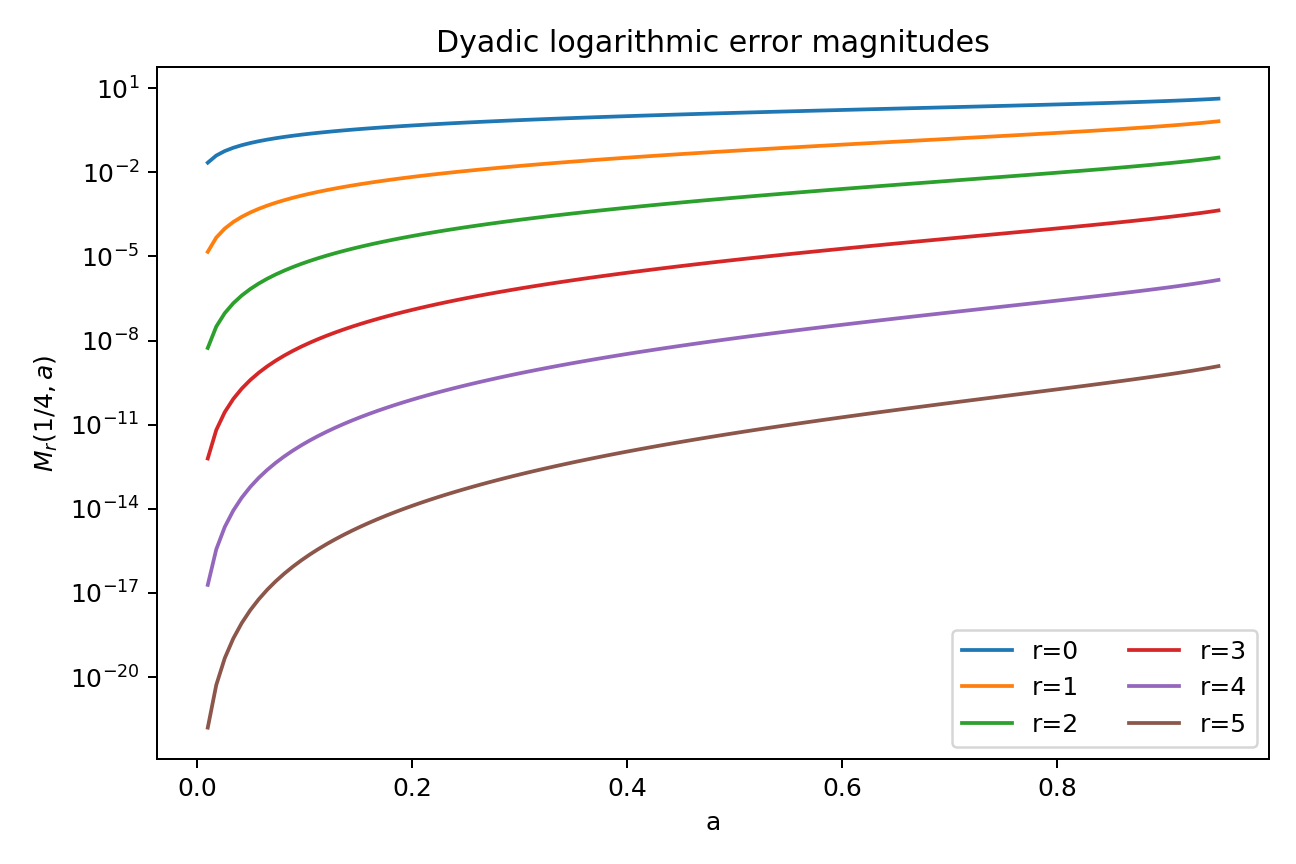
\includegraphics[width=0.86\textwidth]{figures/dyadic_error_magnitudes.png}
\caption{The dyadic magnitudes $M_r(1/4,a)$ for $0.01\le a\le0.95$.  Each parity is
strictly nested over the whole interval, as guaranteed by
\cref{thm:nesting-classification}.  The vertical scale is logarithmic.}
\label{fig:dyadic-errors}
\end{figure}

The separation is dramatic: cancellation order increases by two powers of $a$ each time,
while the prefactor contributes the additional supergeometric factor $q^{r(r+1)/2}$.

\subsection{Unique reversal beyond the threshold}

\begin{figure}[htbp]
\centering
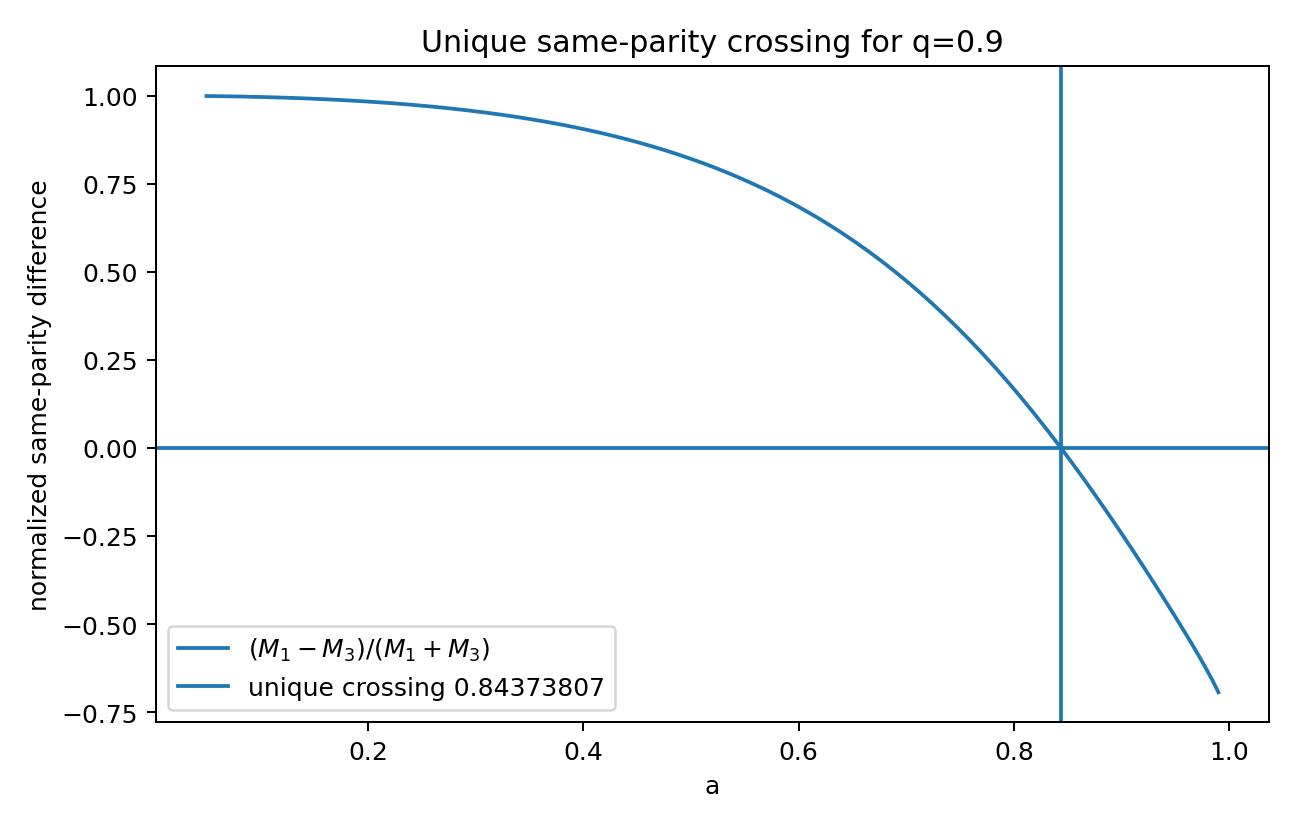
\includegraphics[width=0.86\textwidth]{figures/unique_same_parity_crossing.png}
\caption{For $q=0.9$ and $r=1$, uniform nesting fails.  The normalized difference between
$M_1$ and $M_3$ crosses zero exactly once, at
$a_1(0.9)=0.843738074718284\ldots$.}
\label{fig:crossing}
\end{figure}

Representative crossing values are
\begin{center}
\begin{tabular}{@{}ccr@{}}
\toprule
$q$ & $r$ & $a_r(q)$\\
\midrule
0.7 & 0 & 0.999706476977084941\\
0.8 & 0 & 0.982411424014939233\\
0.8 & 1 & 0.980062142113792208\\
0.9 & 0 & 0.938630662551898552\\
0.9 & 1 & 0.843738074718284012\\
0.9 & 2 & 0.847999350512777102\\
0.9 & 3 & 0.887485076384088108\\
\bottomrule
\end{tabular}
\end{center}
The roots are numerical illustrations only; existence and uniqueness are proved without
numerics.

\subsection{A multiplicity-five zero}

Take $m=48$, whose zero multiplicity is $1+\nu_2(48)=5$, and choose $N=5$, so
$|m|<2^6$.  The exact positive tail is
\[
 \mathcal T_5(48)=\Phi(48/64)=0.217723205308944050125343\ldots.
\]
By \eqref{eq:dyadic-derivative-ratio}, every tail ratio below is exactly the ratio of the
first nonzero derivative of the approximation to $\Phi^{(5)}(48)$.

\begin{center}
\small
\begin{tabular}{@{}rlll@{}}
\toprule
$r$ & derivative ratio & signed log error & side\\
\midrule
0 & 4.592987681680617293 & $+1.524530723363272884$ & upper\\
1 & 0.922841469541933824 & $-8.0297814873516\,10^{-2}$ & lower\\
2 & 1.001952802143219852 & $+1.9508979037801\,10^{-3}$ & upper\\
3 & 0.999986570110615447 & $-1.3429979566325\,10^{-5}$ & lower\\
4 & 1.000000024414975206 & $+2.4414974907466\,10^{-8}$ & upper\\
5 & 0.999999999988534678 & $-1.1465321627915\,10^{-11}$ & lower\\
6 & 1.000000000000001377 & $+1.3766098031980\,10^{-15}$ & upper\\
8 & 1.000000000000000000000000325 & $+3.24694\,10^{-25}$ & upper\\
\bottomrule
\end{tabular}
\end{center}

\begin{figure}[htbp]
\centering
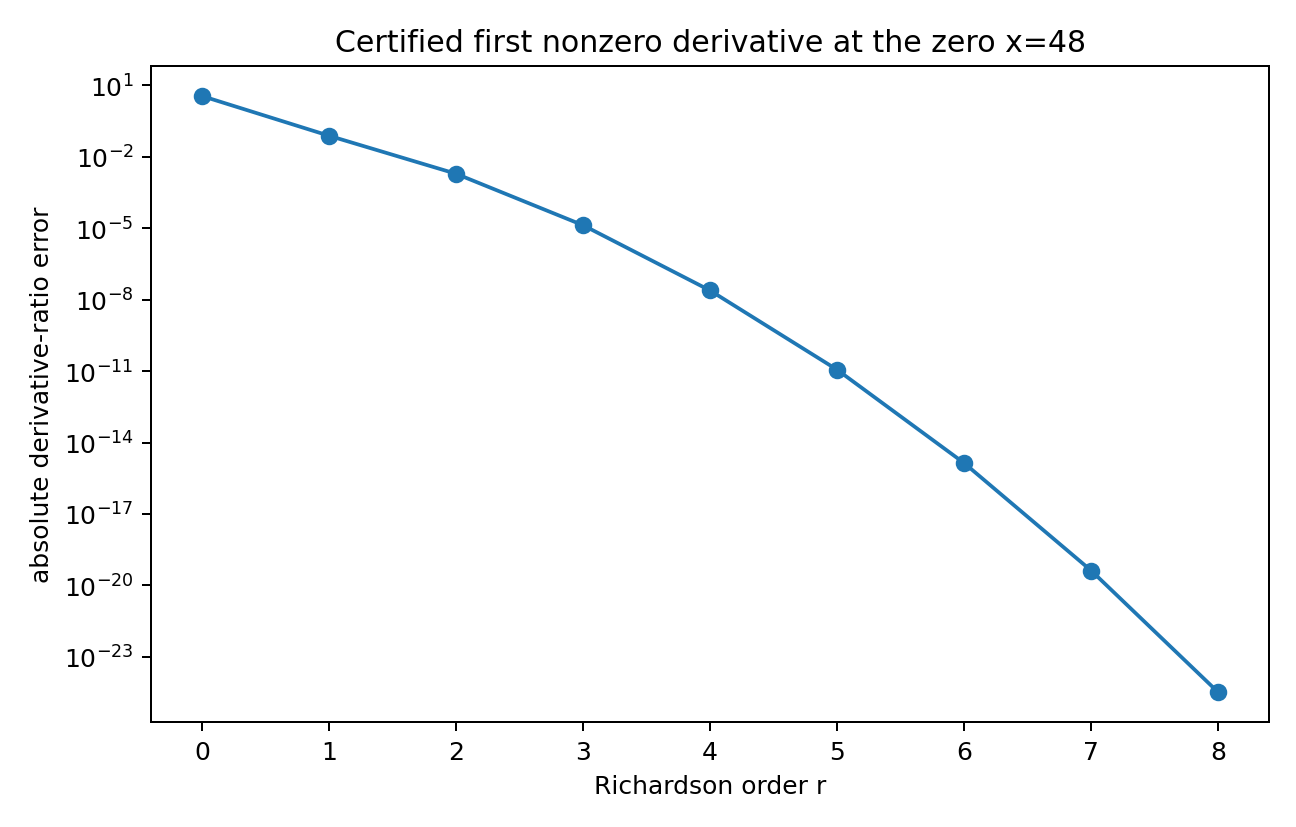
\includegraphics[width=0.86\textwidth]{figures/integer_zero_derivative_convergence.png}
\caption{Absolute error in the certified first-nonzero-derivative ratio at the integer zero
$x=48$.  The factorized construction is well-conditioned here because no logarithm of the
vanishing full product is taken.}
\label{fig:zero-derivative}
\end{figure}

\section{Conjectures and frontier directions}\label{sec:future}

The two exact theorems above close specific open items in the current repository, but they
also expose several more structured questions.

\begin{conjecture}[Regular-variation universality]\label{conj:regular-variation}
Let an even analytic refinement factor satisfy
$-\Log f(z)=\sum_{m\ge1}c_mz^{2m}$ with $c_m>0$ and
$c_m\sim C\rho^{-m}/m$ for some $C,\rho>0$.  After normalizing the tail variable so that the
first logarithmic singularity occurs at $a=1$, the exact same-parity classification remains
$q^{r+1}(1+q)\le1$, with one unique crossing in the supercritical regime.
\end{conjecture}

The sinc proof strongly suggests this: coefficientwise sufficiency is already universal by
\cref{prop:universal-mask}, and regular variation should reproduce the logarithmic boundary
term needed for necessity.

\begin{conjecture}[Monotonicity of the crossing curve]\label{conj:crossing-curve}
For each fixed $r$, the supercritical crossing $a_r(q)$ decreases from $1$ as
$q\downarrow q_r$ and has a finite, strictly positive limit as $q\uparrow1$.  A useful
sharpening would determine the two endpoint asymptotic expansions explicitly.
\end{conjecture}

The first limit follows qualitatively from compact convergence and the threshold theorem;
the monotonicity and the $q\uparrow1$ scale remain to be proved.  The numerical values show
that dependence on $r$ is not simply monotone, so a two-parameter saddle analysis is likely
needed.

\begin{problem}[Optimal finite-precision order]\label{prob:finite-precision}
Given $q$, tail radius $a$, and working precision $p$, determine the order $r$ minimizing a
rigorous sum of truncation, logarithm-evaluation, argument-reduction, and rounding errors.
For $q=1/4$, the exact weight condition number remains bounded, so one expects an optimal
order growing roughly like a square root of $p$ after the supergeometric
$q^{r(r+1)/2}$ factor is balanced against finite-precision noise.
\end{problem}

\begin{problem}[Complex boundary continuation]\label{prob:complex-boundary}
The factorized transform is optimal inside the first omitted zero circle.  Extend it across
that boundary by moving the newly encountered canonical factors from the tail into the
prefix.  The goal is an analytic continuation algorithm with overlapping disks, explicit
transition maps, and uniform Cauchy certificates on arbitrary compact subsets of $\C$.
\end{problem}

This should be feasible because adjacent factorizations differ by finitely many exact sinc
factors.  The delicate point is choosing normalized logarithms coherently on overlaps.

\begin{problem}[Pascal--Rvachev hierarchy]\label{prob:pascal}
For the hierarchy whose Fourier products carry Pascal weights at dyadic scales, construct
confluent or multivariate $q$-Richardson filters that cancel the polynomial-in-scale
multiplicity structure.  Determine whether their same-parity thresholds factor into simple
inequalities analogous to $q^{r+1}(1+q)\le1$.
\end{problem}

\begin{problem}[Inverse-Fabius coupling]\label{prob:inverse-coupling}
Use zero-preserving Fourier brackets as certified inputs to the inverse-Fabius saddle
calculation.  The target is a fully rigorous end-to-end interval algorithm for inverse
values in which Lambert phase, periodic corrections, Fourier amplitudes, and all local zero
jets carry compatible error enclosures.
\end{problem}

\begin{conjecture}[Resurgent organization of phase coefficients]\label{conj:resurgence}
The all-orders inverse endpoint coefficients, after exact phase locking, admit a Borel
transform whose nearest singularities are controlled by the same dyadic complex lattice
that governs the Mellin poles and zero-divisor heat trace.  If true, optimal truncation and
exponentially improved remainders would be determined by one shared spectral geometry.
\end{conjecture}

\begin{problem}[Automatic arithmetic of extrapolated jets]\label{prob:automatic-jets}
At integer and half-integer arguments, investigate whether suitably normalized coefficients
of the factorized approximants form $2$-regular or $2$-automatic arrays.  The finite prefix
has explicit Thue--Morse/Pascal arithmetic, while the tail weights are Gaussian
$q$-binomials at $q=1/4$; their interaction may produce new exact recurrences.
\end{problem}

\section{Lean formalization blueprint}\label{sec:lean}

The proof dependencies are unusually clean.  A sensible formalization order is:
\begin{enumerate}
\item finite $q$-Pochhammer algebra and the closed weights \eqref{eq:weights};
\item the transformed-moment identity \eqref{eq:transformed-moments};
\item positivity and monotonicity of $R_{r,m}$;
\item the algebraic equivalence \eqref{eq:threshold-equivalence};
\item coefficientwise sufficiency;
\item the accelerated boundary decomposition \eqref{eq:accelerated-M};
\item the one-sign-change power-series lemma and unique crossing;
\item analytic zero-free logarithms on a disk;
\item the factorized transform and common-zero-divisor theorem;
\item specialization to the existing Rvachev Fourier product and integer multiplicity API.
\end{enumerate}

The same-parity theorem is mostly finite algebra plus positive series and should be the easier
half.  The factorized continuation needs complex analysis but avoids branch ambiguity by
using a simply connected disk and logarithms normalized at zero.  Existing Lean declarations
for the Rvachev product, scaling, and integer zeros should make the final specialization
short.

\section{Conclusion}

The mature Fabius-function corpus leaves little room for novelty by relabeling familiar
identities.  The productive route was to take two explicit open defects in its newest
$q$-Richardson analysis seriously.

Factoring the finite prefix changes the analytic status of the extrapolator: it becomes a
holomorphic, zero-divisor-preserving approximation on the entire natural disk, not merely a
formula between zeros.  The error series survives unchanged, so all Bernoulli, Bell, and
$q$-binomial structure transfers directly to local spectral jets.  Separately, comparing
same-parity coefficient arrays yields a complete and unexpectedly simple threshold,
$q^{r+1}(1+q)\le1$, together with a one-crossing theorem when it fails.

For the dyadic Rvachev product the consequence is especially clean.  Since $q=1/4$ lies far
inside the golden-ratio threshold, every order participates in two monotone analytic chains.
They squeeze the product, preserve every included integer zero and its Thue--Morse lobe sign,
and certify the first nonzero derivative at multiple zeros to arbitrarily high precision.
This turns the existing extrapolation machinery into a global spectral tool and provides a
compact target for formal verification.

\appendix

\section{Complete recursive TeX manifest}\label{app:manifest}

The following manifest is included verbatim from \path{corpus_manifest.txt}.  The first four
metadata lines are followed by the 68 unique paths used in the audit.

\begingroup
\small
\setlength{\LTpre}{0.4em}
\setlength{\LTpost}{0em}
\begin{longtable}{@{}p{\textwidth}@{}}
\toprule
\textbf{Repository:} VladimirReshetnikov/ProveIt\\
\textbf{Pinned commit:} \nolinkurl{7f4e6e6fdd57f756f303b20f56b5382627e5e1d4}\\
\textbf{Subtree:} \path{Analysis/FabiusFunction/docs}\\
\textbf{TeX files:} 68\\[0.25em]
\midrule
\endfirsthead
\multicolumn{1}{c}{\small\itshape Recursive TeX manifest (continued)}\\[0.25em]
\toprule
\endhead
\midrule
\multicolumn{1}{r}{\small\itshape Continued on the next page}\\
\endfoot
\bottomrule
\endlastfoot
\nolinkurl{Analysis/FabiusFunction/docs/FabiusFunction_Mathematical_Glossary/FabiusFunction_Mathematical_Glossary.tex}\\[0.12em]
\nolinkurl{Analysis/FabiusFunction/docs/Fabius_Function_and_Rvachev_Up/Fabius_Function_and_Rvachev_Up.tex}\\[0.12em]
\nolinkurl{Analysis/FabiusFunction/docs/Non_Elementarity_of_the_Fabius_Function/Non_Elementarity_of_the_Fabius_Function.tex}\\[0.12em]
\nolinkurl{Analysis/FabiusFunction/docs/fabius_lean_walkthrough/fabius_lean_walkthrough.tex}\\[0.12em]
\nolinkurl{Analysis/FabiusFunction/docs/non-formalized-research-frontiers/non-formalized-research-frontiers.tex}\\[0.12em]
\nolinkurl{Analysis/FabiusFunction/docs/non-formalized-research-frontiers/drafts/Fabius_Arithmetic_Rays_Frontier_Report/Fabius_Arithmetic_Rays_Frontier_Report.tex}\\[0.12em]
\nolinkurl{Analysis/FabiusFunction/docs/non-formalized-research-frontiers/drafts/Fabius_Half_Integer_Spectral_Frontier_Report/Fabius_Half_Integer_Spectral_Frontier_Report.tex}\\[0.12em]
\nolinkurl{Analysis/FabiusFunction/docs/non-formalized-research-frontiers/drafts/Fabius_Inverse_Frontier_Report_Source_and_PDF/Fabius_Inverse_Frontier_Report.tex}\\[0.12em]
\nolinkurl{Analysis/FabiusFunction/docs/non-formalized-research-frontiers/drafts/Fabius_Rvachev_Frontier_Report-2/Fabius_Rvachev_Frontier_Report.tex}\\[0.12em]
\nolinkurl{Analysis/FabiusFunction/docs/non-formalized-research-frontiers/drafts/Fabius_Rvachev_Frontier_Report/Fabius_Rvachev_Frontier_Report.tex}\\[0.12em]
\nolinkurl{Analysis/FabiusFunction/docs/non-formalized-research-frontiers/drafts/Fabius_Rvachev_New_Frontiers/Fabius_Rvachev_New_Frontiers.tex}\\[0.12em]
\nolinkurl{Analysis/FabiusFunction/docs/non-formalized-research-frontiers/drafts/Fabius_Rvachev_Thue_Morse_Frontier_Results/Fabius_Rvachev_Thue_Morse_Frontier_Results.tex}\\[0.12em]
\nolinkurl{Analysis/FabiusFunction/docs/non-formalized-research-frontiers/drafts/Spectral_Arithmetic_Pascal_Rvachev_Hierarchy/Spectral_Arithmetic_Pascal_Rvachev_Hierarchy.tex}\\[0.12em]
\nolinkurl{Analysis/FabiusFunction/docs/non-formalized-research-frontiers/drafts/Thue_Morse_Formula_Atlas/Thue_Morse_Formula_Atlas.tex}\\[0.12em]
\nolinkurl{Analysis/FabiusFunction/docs/non-formalized-research-frontiers/drafts/fabius_frontier_new_results/fabius_frontier_new_results.tex}\\[0.12em]
\nolinkurl{Analysis/FabiusFunction/docs/non-formalized-research-frontiers/drafts/fabius_frontier_results_bundle/fabius_frontier_results.tex}\\[0.12em]
\nolinkurl{Analysis/FabiusFunction/docs/non-formalized-research-frontiers/drafts/fabius_frontier_spectral_endpoint_report_bundle/fabius_frontier_spectral_endpoint_report.tex}\\[0.12em]
\nolinkurl{Analysis/FabiusFunction/docs/non-formalized-research-frontiers/drafts/rvachev_up_fourier_decay/Rvachev_Up_Fourier_Decay-2/Rvachev_Up_Fourier_Decay.tex}\\[0.12em]
\nolinkurl{Analysis/FabiusFunction/docs/non-formalized-research-frontiers/drafts/rvachev_up_fourier_decay/Rvachev_Up_Fourier_Decay-3/Fourier_decay_of_Rvachev_up.tex}\\[0.12em]
\nolinkurl{Analysis/FabiusFunction/docs/non-formalized-research-frontiers/drafts/rvachev_up_fourier_decay/Rvachev_Up_Fourier_Decay_Comparative_Audit/Rvachev_Up_Fourier_Decay_Comparative_Audit.tex}\\[0.12em]
\nolinkurl{Analysis/FabiusFunction/docs/non-formalized-research-frontiers/drafts/rvachev_up_fourier_decay/Rvachev_Up_Fourier_Decay_Gentle_Guide/Rvachev_Up_Fourier_Decay_Gentle_Guide.tex}\\[0.12em]
\nolinkurl{Analysis/FabiusFunction/docs/non-formalized-research-frontiers/drafts/rvachev_up_fourier_decay/Rvachev_Up_Fourier_Decay_Second_Wave_Audit/Rvachev_Up_Fourier_Decay_Second_Wave_Audit.tex}\\[0.12em]
\nolinkurl{Analysis/FabiusFunction/docs/non-formalized-research-frontiers/drafts/rvachev_up_fourier_decay/asymptotic-decay-rate-of-an-infinite-product-of-sinc-functions/asymptotic-decay-rate-of-an-infinite-product-of-sinc-functions.tex}\\[0.12em]
\nolinkurl{Analysis/FabiusFunction/docs/non-formalized-research-frontiers/drafts/rvachev_up_fourier_decay/rvachev_up_fourier_decay-1/rvachev_up_fourier_decay.tex}\\[0.12em]
\nolinkurl{Analysis/FabiusFunction/docs/non-formalized-research-frontiers/drafts/rvachev_up_fourier_decay/rvachev_up_fourier_decay-4/rvachev_up_fourier_decay.tex}\\[0.12em]
\nolinkurl{Analysis/FabiusFunction/docs/non-formalized-research-frontiers/drafts/rvachev_up_fourier_decay/rvachev_up_fourier_decay-5/Rvachev_Up_Fourier_Decay_Final.tex}\\[0.12em]
\nolinkurl{Analysis/FabiusFunction/docs/non-formalized-research-frontiers/drafts/rvachev_up_fourier_decay/rvachev_up_fourier_decay-6/Rvachev_Up_Fourier_Decay_Final_Synthesis.tex}\\[0.12em]
\nolinkurl{Analysis/FabiusFunction/docs/non-formalized-research-frontiers/drafts/rvachev_up_fourier_decay/rvachev_up_fourier_decay-7/rvachev_up_fourier_decay_final.tex}\\[0.12em]
\nolinkurl{Analysis/FabiusFunction/docs/non-formalized-research-frontiers/drafts/rvachev_up_fourier_decay/rvachev_up_fourier_decay-8/rvachev_up_fourier_decay_final.tex}\\[0.12em]
\nolinkurl{Analysis/FabiusFunction/docs/archive/early-notes/Fabius Asymptotic/Fabius Asymptotic.tex}\\[0.12em]
\nolinkurl{Analysis/FabiusFunction/docs/archive/early-notes/K-fold summation over the signed Thue-Morse sequence/K-fold summation over the signed Thue-Morse sequence.tex}\\[0.12em]
\nolinkurl{Analysis/FabiusFunction/docs/archive/glossary/FabiusFunction_Mathematical_Glossary-2/FabiusFunction_Mathematical_Glossary.tex}\\[0.12em]
\nolinkurl{Analysis/FabiusFunction/docs/archive/glossary/FabiusFunction_Mathematical_Glossary/FabiusFunction_Mathematical_Glossary.tex}\\[0.12em]
\nolinkurl{Analysis/FabiusFunction/docs/archive/lean-walkthrough/Fabius_Function_Lean_Walkthrough/Fabius_Function_Lean_Walkthrough.tex}\\[0.12em]
\nolinkurl{Analysis/FabiusFunction/docs/archive/lean-walkthrough/fabius_lean_walkthrough/fabius_lean_walkthrough.tex}\\[0.12em]
\nolinkurl{Analysis/FabiusFunction/docs/archive/primary-exposition/Fabius_Function_and_Rvachev_Up-2/Fabius_Function_and_Rvachev_Up.tex}\\[0.12em]
\nolinkurl{Analysis/FabiusFunction/docs/archive/primary-exposition/Fabius_Function_and_Rvachev_Up-3/Fabius_Function_and_Rvachev_Up.tex}\\[0.12em]
\nolinkurl{Analysis/FabiusFunction/docs/archive/primary-exposition/Fabius_Function_and_Rvachev_Up/Fabius_Function_and_Rvachev_Up.tex}\\[0.12em]
\nolinkurl{Analysis/FabiusFunction/docs/archive/primary-exposition/Fabius_and_Rvachev_Up-2/Fabius_and_Rvachev_Up.tex}\\[0.12em]
\nolinkurl{Analysis/FabiusFunction/docs/archive/primary-exposition/Fabius_and_Rvachev_up/Fabius_and_Rvachev_up.tex}\\[0.12em]
\nolinkurl{Analysis/FabiusFunction/docs/archive/primary-exposition/Fabius_function_and_up_function/Fabius_function_and_up_function.tex}\\[0.12em]
\nolinkurl{Analysis/FabiusFunction/docs/archive/primary-supplements/Fabius_Function_Missing_Parts-2/Fabius_Function_Missing_Parts.tex}\\[0.12em]
\nolinkurl{Analysis/FabiusFunction/docs/archive/primary-supplements/Fabius_Function_Missing_Parts/Fabius_Function_Missing_Parts.tex}\\[0.12em]
\nolinkurl{Analysis/FabiusFunction/docs/archive/q-calculus/Fabius_q_Special_Functions/Fabius_q_Special_Functions.tex}\\[0.12em]
\nolinkurl{Analysis/FabiusFunction/docs/archive/q-calculus/fabius-q-special-functions/fabius-q-special-functions.tex}\\[0.12em]
\nolinkurl{Analysis/FabiusFunction/docs/archive/research-frontiers/Fabius_Dyadic_Asymptotic_Bridge/Fabius_Dyadic_Asymptotic_Bridge.tex}\\[0.12em]
\nolinkurl{Analysis/FabiusFunction/docs/archive/research-frontiers/Fabius_Dyadic_Formulae_and_Alternative_Representations/Fabius_Dyadic_Formulae_and_Alternative_Representations.tex}\\[0.12em]
\nolinkurl{Analysis/FabiusFunction/docs/archive/research-frontiers/Fabius_Dyadic_Formulae_to_Asymptotics/Fabius_Dyadic_Formulae_to_Asymptotics.tex}\\[0.12em]
\nolinkurl{Analysis/FabiusFunction/docs/archive/research-frontiers/Fabius_Dyadic_q_Connections/Fabius_Dyadic_q_Connections.tex}\\[0.12em]
\nolinkurl{Analysis/FabiusFunction/docs/archive/research-frontiers/Fabius_Thue_Morse_Convergence_Rate/Fabius_Thue_Morse_Convergence_Rate.tex}\\[0.12em]
\nolinkurl{Analysis/FabiusFunction/docs/archive/research-frontiers/Fabius_Thue_Morse_Convergence_Rates/Fabius_Thue_Morse_Convergence_Rates.tex}\\[0.12em]
\nolinkurl{Analysis/FabiusFunction/docs/archive/research-frontiers/Primary_Exposition_Gap_Register/Primary_Exposition_Gap_Register.tex}\\[0.12em]
\nolinkurl{Analysis/FabiusFunction/docs/archive/research-frontiers/Repeated_Integration_and_Rvachev_Up/Repeated_Integration_and_Rvachev_Up.tex}\\[0.12em]
\nolinkurl{Analysis/FabiusFunction/docs/archive/research-frontiers/Rvachev_Up_from_Repeated_Integration/Rvachev_Up_from_Repeated_Integration.tex}\\[0.12em]
\nolinkurl{Analysis/FabiusFunction/docs/archive/research-frontiers/Thue_Morse_Formula_Atlas-1/Thue_Morse_Formula_Atlas.tex}\\[0.12em]
\nolinkurl{Analysis/FabiusFunction/docs/archive/research-frontiers/Thue_Morse_Formula_Atlas-2/Consolidated_Formula_Atlas_for_the_Thue_Morse_Sequence.tex}\\[0.12em]
\nolinkurl{Analysis/FabiusFunction/docs/archive/research-frontiers/Thue_Morse_Formula_Atlas-3/Thue_Morse_Formula_Atlas.tex}\\[0.12em]
\nolinkurl{Analysis/FabiusFunction/docs/archive/research-frontiers/non-formalized-research-frontiers/non-formalized-research-frontiers.tex}\\[0.12em]
\nolinkurl{Analysis/FabiusFunction/docs/archive/standalone-studies/Non_Elementarity_of_the_Fabius_Function/Non_Elementarity_of_the_Fabius_Function.tex}\\[0.12em]
\nolinkurl{Analysis/FabiusFunction/docs/archive/standalone-studies/Small_Argument_Asymptotics/Small_Argument_Asymptotics.tex}\\[0.12em]
\nolinkurl{Analysis/FabiusFunction/docs/archive/standalone-studies/fabius-inverse-dyadic-closed-form/fabius-inverse-dyadic-closed-form.tex}\\[0.12em]
\nolinkurl{Analysis/FabiusFunction/docs/papers/AIF_2017__67_2_637_0/AIF_2017__67_2_637_0-corrected.tex}\\[0.12em]
\nolinkurl{Analysis/FabiusFunction/docs/papers/AIF_2017__67_2_637_0/AIF_2017__67_2_637_0.tex}\\[0.12em]
\nolinkurl{Analysis/FabiusFunction/docs/papers/arXiv-1502.06738v2/Lacunary_products.tex}\\[0.12em]
\nolinkurl{Analysis/FabiusFunction/docs/papers/arXiv-1702.05442v1/09-Function.tex}\\[0.12em]
\nolinkurl{Analysis/FabiusFunction/docs/papers/arXiv-1702.06487v3/157-Arithmetic-v3.tex}\\[0.12em]
\nolinkurl{Analysis/FabiusFunction/docs/papers/arXiv-2211.13570v1/document.tex}\\[0.12em]
\nolinkurl{Analysis/FabiusFunction/docs/papers/ubiq15/ubiq15-corrected.tex}\\[0.12em]
\end{longtable}
\endgroup


\section{Reproduction files}\label{app:files}

The ZIP archive accompanying this report contains:
\begin{longtable}{@{}p{0.42\textwidth}p{0.52\textwidth}@{}}
\toprule
Path & Purpose\\
\midrule
\endhead
\path{fabius_frontier_report.tex} & Complete LaTeX source.\\
\path{fabius_frontier_report.pdf} & Rendered report.\\
\path{code/frontier_experiments.py} & Fully commented numerical experiment and figure generator.\\
\path{data/same_parity_thresholds.csv} & Threshold roots $q_r$ and bases $b_r$.\\
\path{data/same_parity_crossings.csv} & Representative unique crossing roots.\\
\path{data/dyadic_q_richardson_weights.csv} & Low-order geometric Lagrange weights.\\
\path{data/integer_zero_jet_brackets.csv} & Certified derivative-ratio experiment at $x=48$.\\
\path{data/nonzero_point_factorized_errors.csv} & Direct product/series cross-check away from zeros.\\
\path{figures/*.png} & The three figures embedded above.\\
\path{corpus_manifest.txt} & Pinned recursive source inventory.\\
\path{corpus_manifest_table.tex} & Breakable LaTeX rendering of the inventory used by Appendix~\ref{app:manifest}.\\
\path{experiment_summary.txt} & Compact numerical run summary.\\
\path{requirements.txt} & Python dependency bounds.\\
\path{README.md} & Reproduction and file guide.\\
\path{SHA256SUMS} & SHA-256 checksums for packaged files.\\
\bottomrule
\end{longtable}

\begin{thebibliography}{99}

\bibitem{repo}
V. Reshetnikov,
\emph{ProveIt: Analysis/FabiusFunction documentation corpus},
GitHub repository, snapshot \commitsha,
\url{https://github.com/VladimirReshetnikov/ProveIt/tree/7f4e6e6fdd57f756f303b20f56b5382627e5e1d4/Analysis/FabiusFunction/docs}.

\bibitem{arias-function}
J. Arias de Reyna,
\emph{An infinitely differentiable function with compact support: definition and properties},
arXiv:1702.05442, English translation of Rev. Real Acad. Cienc. Exactas Fis. Nat. 76 (1982), 21--38.

\bibitem{arias-arithmetic}
J. Arias de Reyna,
\emph{Arithmetic of the Fabius function},
arXiv:1702.06487, 2017.

\bibitem{haugland}
J. K. Haugland,
\emph{Evaluating the Fabius function},
arXiv:1609.07999, 2016.

\bibitem{ahl2017}
C. Aistleitner, R. Hofer, and G. Larcher,
\emph{On evil Kronecker sequences and lacunary trigonometric products},
Ann. Inst. Fourier (Grenoble) 67 (2017), no. 2, 637--687.

\bibitem{allouche-shallit}
J.-P. Allouche and J. Shallit,
\emph{The ubiquitous Prouhet--Thue--Morse sequence},
in Sequences and Their Applications, Springer, 1999, 1--16.

\bibitem{toth}
L. Toth,
\emph{Linear combinations of Dirichlet series associated with the Thue--Morse sequence},
arXiv:2211.13570, 2022.

\bibitem{gasper-rahman}
G. Gasper and M. Rahman,
\emph{Basic Hypergeometric Series}, 2nd ed.,
Encyclopedia of Mathematics and its Applications 96, Cambridge University Press, 2004,
\doi{10.1017/CBO9780511526251}.

\bibitem{sidi1996}
A. Sidi,
\emph{Further results on convergence and stability of a generalization of the Richardson extrapolation process},
BIT Numerical Mathematics 36 (1996), 143--157,
\doi{10.1007/BF01740551}.

\bibitem{sidi-siam}
A. Sidi,
\emph{A complete convergence and stability theory for a generalized Richardson extrapolation process},
SIAM J. Numer. Anal. 34 (1997), 1761--1778,
\doi{10.1137/S0036142994278589}.

\bibitem{corless}
R. M. Corless, G. H. Gonnet, D. E. G. Hare, D. J. Jeffrey, and D. E. Knuth,
\emph{On the Lambert $W$ function},
Advances in Computational Mathematics 5 (1996), 329--359,
\doi{10.1007/BF02124750}.

\bibitem{comtet}
L. Comtet,
\emph{Advanced Combinatorics: The Art of Finite and Infinite Expansions},
D. Reidel, 1974.

\end{thebibliography}

\end{document}
